Suppose we sample from a random variable $X$ with image $\cal X$. In the context of data compression, $X$ is typically called a \term{source} that `spits out' the value $x \in {\cal X}$ with probability $P_X(x)$. We want to compress (or encode) $x$ in such a way that we can later decompress (or decode) it reliably, without losing any information about the value $x$.

\begin{figure}[h]
\begin{center}
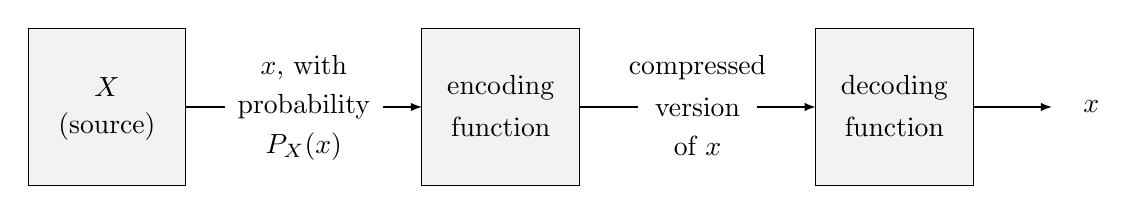
\begin{tikzpicture}
\draw[fill=black!5] (0,0) rectangle (2,2);
\node at (1,1.25) {$X$};
\node at (1,0.75) {(source)};

\draw[-latex] (2,1) -- (5,1);
\draw[fill=white,draw=none] (2.5,0) rectangle (4.5,2);
\node at (3.5,1.5) {$x$, with};
\node at (3.5,1) {probability};
\node at (3.5,0.5) {$P_X(x)$};

\draw[fill=black!5] (5,0) rectangle (7,2);
\node at (6,1.25) {encoding};
\node at (6,0.75) {function};

\draw[-latex] (7,1) -- (10,1);
\draw[fill=white,draw=none] (7.75,0) rectangle (9.25,2);
\node at (8.5,1.5) {compressed};
\node at (8.5,1) {version};
\node at (8.5,0.5) {of $x$};

\draw[fill=black!5] (10,0) rectangle (12,2);
\node at (11,1.25) {decoding};
\node at (11,0.75) {function};

\draw[-latex] (12,1) -- (13,1);
\node at (13.5,1) {$x$};
\end{tikzpicture}
\end{center}
\end{figure}

\noindent A counting argument shows that it is possible to encode the elements of ${\cal X}$ by bit strings of length $n$, where $n=\lceil \log (|{\cal X}|) \rceil $: we simply list all elements of ${\cal X}$, and use the index of $x$ in the list as its encoding. 
Thus, to store or to transmit an element $x\in {\cal X}$, $n$ bits
of information always suffice. However, if not all $x \in \cal X$ are equally likely with respect to $X$, one should be able to
exploit this to achieve codes with shorter {\em average} length. The idea is to use encodings of varying lengths, assigning shorter codewords to the elements in ${\cal X}$ that have higher probabilities, and vice versa.
The question we answer in this chapter is: how short can such a code be (on average over the choice of~$x$)?

We explore both \term{lossless} codes (where we want to recover the original data with certainty) and \term{lossy} codes (where with small probability, the data is lost).
%The average length of the code is inversely related the amount of information that is contained in $X$.


%Let $X$ be a random variable with image $\cal X$. A counting argument shows that it is possible to encode the elements of ${\cal X}$ by bit strings of length $n$, where $n=\lceil \log (|{\cal X}|) \rceil $: we simply list all elements of ${\cal X}$, and use the binary representation of their index in the list as the encoding. 
%Thus, to store or to transmit an element $x\in {\cal X}$, $n$ bits
%of information always suffice. However, if not all $x \in \cal X$ are equally likely with respect to $X$ (in this context typically called the \term{source}), one should be able to
%exploit this to achieve codes with shorter {\em expected} length. The idea is to use encodings of varying lengths, assigning shorter codewords to the elements in ${\cal X}$ that have higher probabilities, and vice versa.
%The question we answer in this chapter is: how short can such a code be (on average over the choice of~$x$)?




\section{Symbol codes}
We start by investigating codes that encode a source one symbol as a time. Later on, we will also see codes that group the source symbols together into blocks.
\begin{definition}[Binary symbol code]
Let $X$ be a random variable with image ${\cal X}$. A binary symbol code for $X$ is an injective function $C : {\cal X} \to \strg$.

The \term{extended} code $C^* : {\cal X}^* \to \strg$ is defined by concatenation:
\[
C^*(x_1, ..., x_n) := C(x_1) | \cdots |C(x_n).
\]
Here, ${\cal X}^* = \bigcup_{n \in \N} {\cal X}^n \cup \set{\es}$, and $\es$ is the empty string.
\end{definition}
We often refer to the set of codewords, ${\cal C} = \im(C)$, as code and leave the actual encoding function $C$ implicit. 

The injectivity of $C$ ensures that we can always uniquely decode $C(x)$. However, if one transmits a sequence $x_1, \ldots, x_m\in {\cal X}$
(or stores them ``sequentially'') by sending the concatenation $C(x_1, ..., x_n)$, ambiguities may arise, namely in cases where it is possible to parse this long
string in two consistent but different ways. Indeed, injectivity of
the encoding function per se does not rule out that there exists a
positive integer $m'$ and elements $x'_1, \ldots, x'_{m'}\in {\cal X}$
such that $C(x_1)| \cdots | C(x_m)=C(x'_1)| \cdots | C(x'_{m'})$. Of course, this problem can be circumvented by introducing a special separation symbol. However, such a symbol might not be available, and maybe even more importantly, even if an additional symbol {\em is} available, then one can often create a better code by using it as an ordinary code symbol (in addition to 0 and 1) rather than as a special separation symbol. This is why it is interesting to study the following class of symbol codes:

\begin{definition}[Uniquely decodable code]
A binary symbol code $C : {\cal X} \to \strg$ is uniquely decodable if $C^*$ is injective as well.
\end{definition}

One convenient way to guarantee that a code is unique decodable is to require it to be prefix-free:
\begin{definition}[Prefix-free code]
A binary symbol code $C : {\cal X} \to \strg$ is prefix-free (or: \term{instantaneous}) if for all $x, x' \in \cal X$ with $x \neq x'$, $C(x)$ is {\em not} a prefix of $C(x')$.
\end{definition}

With a prefix-free encoding, the elements
$x_1, \ldots, x_m$ can be uniquely recovered from $C(x_1)|\cdots
|C(x_m)$, simply by reading the encoding from left to right one bit
at a time: by prefix-freeness it will remain unambiguous as reading
continues when the current word terminates and the next begins. This is a loose argument for the following:
\begin{proposition}\label{lemma:PF->UD}
If a code $\cal C$ is prefix-free and ${\cal C} \neq \set{\es}$ then $\cal C$ is uniquely decodable. 
\end{proposition}
The other direction does not hold: uniquely decodable codes need not be prefix-free. A prefix-free code is appealing from an efficiency point of view, as it allows to decode ``on the fly''. For a general uniquely decodable code one may possibly have to inspect all bits
in the entire string before being able to even recover the first word. 

\begin{example}\label{example:codes}
The following are three codes for the random variable $X$, with ${\cal X} = \{a,b,c,d\}$:
\[
\begin{array}{c | c | l | l | l}
x & P_X(x) & C_1(x) & C_2(x) & C_3(x)\\
\hline
a & 1/2 & 0   & 0   & 0   \\
\hline
b & 1/4 & 10  & 010 & 01  \\
\hline
c & 1/8 & 110 & 01  & 011 \\
\hline
d & 1/8 & 111 & 10  & 111
\end{array}
\]
These codes can be visualised a as a binary tree, with marked codewords, as follows:
\begin{center}
%C1:
\begin{tikzpicture}
  [
    grow                    = right,
    sibling distance        = 2.5em,
    level distance          = 2.5em,
    edge from parent/.style = {draw},
    every node/.style       = {font=\footnotesize}
  ]
  \node [dummy] {}
    child { node [dummy] {}
      child { node [dummy] {}
        child { node [marked] {}
          edge from parent node [below] {1} }
        child { node [marked] {} 
          edge from parent node [above] {0} }
      	edge from parent node [below] {1} }
      child { node [marked] {} 
        edge from parent node [above] {0} }
      edge from parent node [below] {1} }
    child { node [marked] {}
      edge from parent node [above] {0} };
\end{tikzpicture}
%
\qquad
%
%C2:
\begin{tikzpicture}
  [
    grow                    = right,
    sibling distance        = 2.5em,
    level distance          = 2.5em,
    edge from parent/.style = {draw},
    every node/.style       = {font=\footnotesize}
  ]
  \tikzstyle{level 1}=[sibling distance=5em]
  \tikzstyle{level 2}=[sibling distance=2.5em]
  \node [dummy] {}
    child { node [dummy] {}
      child {node [dummy] {} 
        edge from parent node[below] {1} }
      child {node [marked] {}
        edge from parent node[above] {0} }
      edge from parent node [below] {1} }
    child { node [marked] {}
      child { node [marked] {}
        child { node [dummy] {}
          edge from parent node [below] {1} }
        child { node [marked] {} 
          edge from parent node [above] {0} }
      	edge from parent node [below] {1} }
      child { node [dummy] {} 
        edge from parent node [above] {0} }
      edge from parent node [above] {0} };
\end{tikzpicture}
%
\qquad
%
%C3:
\begin{tikzpicture}
  [
    grow                    = right,
    sibling distance        = 2.5em,
    level distance          = 2.5em,
    edge from parent/.style = {draw},
    every node/.style       = {font=\footnotesize}
  ]
  \node [dummy] {}
    child { node [marked] {}
      edge from parent node [below] {1} }
    child { node [dummy] {}
      child { node [marked] {}
      	edge from parent node [below] {1} }
      child { node [dummy] {} 
        child { node [marked] {}
          edge from parent node [below] {1} }
        child { node [marked] {} 
          edge from parent node [above] {0} }
        edge from parent node [above] {0} }
      edge from parent node [above] {0} };
\end{tikzpicture}
\end{center}
$C_1$ is prefix-free, and therefore also uniquely decodable. $C_2$ is not uniquely decodable, as $C_2(ad) = C_2(b)$.  $C_3$ is not prefix-free, but it is uniquely decodable, since it can be decoded from right to left (it is ``postfix-free"). Note that the binary tree for the prefix-free code $C_1$ only has codewords at the leafs. (The same holds for the postfix-free code $C_3$).
\end{example}
For efficiency reasons, we are often interested in the average (expected) length of a code $C$:
\begin{definition}[Average length]
Let $\len(s)$ denote the length of a string $s \in \strg$. The (average) length of a code $C$ for a source $X$ is defined as
\[
\len_C(X) := E[\len(C(X))] = \sum_{x \in \cal X} P_X(x) \len(C(x)) \, .
\]
\end{definition}
\begin{definition}[Minimal code length]
The minimal code length of a source $X$ is defined as
\[
\len_{\min}(X) := \min_{C \in \frak{C}} \len_C(X)
\]
where $\frak{C}$ is some class of codes, for example the set of all prefix-free codes (resulting in $\len_{\min}^{\text{\rm p.f.}}$), or the set of all uniquely decodable codes (resulting in $\len_{\min}^{\text{\rm u.d.}}$). 
\end{definition}



\section{Kraft's inequality}\label{sec:kraft}
As argued, prefix-freeness is a nice feature, but it is also considerably more restrictive than mere unique decodability; thus, it is natural to ask: how much do we lose (in terms of the average codeword length) by requiring the encoding to be prefix-free rather than merely uniquely decodable? Surprisingly, the answer is: {\em nothing}. In this section, we will show that the length of an optimal prefix-free code and the length of an optimal uniquely decodable code coincide. In the next section, we will see that these lengths are essentially given by the Shannon entropy.

\begin{theorem}[Kraft's inequality]
There exists a prefix-free code with image ${\cal C} = \set{c_1, ..., c_m}$ and codeword lengths $\len_i := \len(c_i)$, if and only if
\[
\sum_{i=1}^m 2^{-\ell_i} \leq 1.
\]
\end{theorem}
\begin{proof}
For the forward direction, suppose we have a prefix-free code $C$ with image ${\cal C} = \set{c_1, ..., c_m}$ and codeword lengths $\len_i := \len(c_i)$. View this code as a tree, with codewords only on the leafs (but not necessarily all the leafs), and assign a weight of $2^{-d}$ to every node in the tree at depth $d$ (including the leafs):
%\begin{figure}[h]
\begin{center}
\begin{tikzpicture}
  [
    grow                    = right,
    sibling distance        = 2.5em,
    level distance          = 2.5em,
    edge from parent/.style = {draw},
    every node/.style       = {font=\footnotesize}
  ]
  
  \draw[dashed] (0,-2) -- (0,2);
  \draw[dashed] (2.5em,-2) -- (2.5em,2);
  \draw[dashed] (5em,-2) -- (5em,2);
  \draw[dashed] (7.5em,-2) -- (7.5em,2);
  \tikzstyle{level 1}=[sibling distance=5em]
  \tikzstyle{level 2}=[sibling distance=2.5em]
  \node [dummy] {}
    child { node [dummy] {}
      child {node [marked] {} 
        edge from parent node[below] {1} }
      child {node [dummy] {}
        child { node [marked] {}
          edge from parent node [below] {1} }
        child { node [marked] {} 
          edge from parent node [above] {0} }
        edge from parent node[above] {0} }
      edge from parent node [below] {1} }
    child { node [dummy] {}
      child { node [dummy] {}
      	edge from parent node [below] {1} }
      child { node [marked] {} 
        edge from parent node [above] {0} }
      edge from parent node [above] {0} };
  \node[anchor=south] at (0    ,2) {$2^0$};
  \node[anchor=south] at (2.5em,2) {$2^{-1}$};
  \node[anchor=south] at (5em  ,2) {$2^{-2}$};
  \node[anchor=south] at (7.5em,2) {$2^{-3}$};
\end{tikzpicture}
\end{center}
%\end{figure}

\noindent Note that the weight of each node is exactly the sum of the weight of its direct children, and thereby that the weight of the root is exactly the weight of all of the leafs. Since every codeword $c_i$ resides on a leaf of depth $\ell_i$ (but not all leafs are necessarily occupied), the weight of the root is \emph{at least} the sum of all the codeword weights:
\begin{align}
\sum_{i=1}^{m} 2^{-\ell_i} \leq 2^0 = 1.
\end{align}

For the backward direction, we build a code ${\cal C} = \{c_1, ..., c_m\}$ with $\ell(c_i) = \len_i$ by selecting the appropriate leafs of a binary tree as codewords, assigning the most `expensive' (i.e. those with small depth) first. We proceed by induction on the number of codewords, $m$:

For $m = 1$, the construction is clear: we can assign any string of length $\len_1$ to represent the single codeword.

For $m > 1$, assume without loss of generality that $\ell_1 \leq \cdots \leq \ell_{m-1} \leq \ell_{m}$. We will first try to build a code with $(m-1)$ code words, of lengths $\ell_1, ..., \ell_{m-2}, (\ell_{m-1} - 1)$. In order to be able to invoke the induction hypothesis, we do need to check that
\begin{align}
\left(\sum_{i=1}^{m-2} 2^{\ell_{i}}\right) + 2^{(\ell_{m-1} - 1)} \leq 1.
\end{align}
This can be seen by first noting that
\begin{align}
1 \ > \ 1 - 2^{-\len_m} \ \geq \ \sum_{i=1}^{m-1} 2^{-\len_i} \ = \ \sum_{i=1}^m \frac{2^{\len_{m-1} - \len_i}}{2^{\len_{m-1}}} \ = \ \frac{\sum_{i=1}^{m-1} 2^{\len_{m-1} - \len_i}}{2^{\len_{m-1}}}.
\end{align}
and then, because both the denominator and the enumerator of the fraction are integers,
\begin{align}
1
\ \geq \ \frac{\left(\sum_{i=1}^{m-1} 2^{\len_{m-1} - \len_i}\right) + 1}{2^{\len_{m-1}}}
&= \ \left(\sum_{i=1}^{m-1} 2^{-\len_i}\right) + 2^{-\len_{m-1}}\nonumber\\
&= \ \left(\sum_{i=1}^{m-2} 2^{-\len_i}\right) + 2\cdot 2^{-\len_{m-1}}\nonumber\\
&= \ \left(\sum_{i=1}^{m-2} 2^{\ell_{i}}\right) + 2^{(\ell_{m-1} - 1)},
\end{align}
as desired. So we invoke the induction hypothesis to create a prefix-free code ${\cal C}' = \{c'_1, ..., c'_{m-1}\}$ with lengths $\len_1, ..., \len_{m-2}, (\len_{m-1} - 1)$. The new code ${\cal C}$ is then constructed by setting $c_i = c'_i$ for all $i \leq m-2$, and furthermore setting $c_{m-1} = c'_{m-1}|0$ and $c_m = c'_{m-1}|10\cdots 0$, padding with enough zeroes to achieve $\len(c_m) = \len_m$. This new code is necessarily also prefix-free.

The following image illustrates the induction step for $\ell_1 = \ell_2 = \ell_3 = 2$ and $\ell_4 = 3$. The code is constructed from a prefix-free code ${\cal C}'$ with code lengths $2, 2$ and 1.

%\begin{figure}[h]
\begin{center}
\begin{tikzpicture}
  [
    grow                    = right,
    sibling distance        = 2.5em,
    level distance          = 2.5em,
    edge from parent/.style = {draw},
    every node/.style       = {font=\footnotesize}
  ]
  \tikzstyle{level 1}=[sibling distance=5em]
  \tikzstyle{level 2}=[sibling distance=2.5em]
  \node [dummy] {}
    child { node [marked] {}
      edge from parent node [below] {1} }
    child { node [dummy] {}
      child { node [marked] {}
      	edge from parent node [below] {1} }
      child { node [marked] {} 
        edge from parent node [above] {0} }
      edge from parent node [above] {0} };
  
  \node[anchor=north] at (2.5em,-2.25) {${\cal C}' = \set{00, 01, 1}$};
\end{tikzpicture}
\qquad
\begin{tikzpicture}
\node at (0,0) {$\Rightarrow$};
\end{tikzpicture}\qquad
\begin{tikzpicture}
  [
    grow                    = right,
    sibling distance        = 2.5em,
    level distance          = 2.5em,
    edge from parent/.style = {draw},
    every node/.style       = {font=\footnotesize}
  ]
  \tikzstyle{level 1}=[sibling distance=5em]
  \tikzstyle{level 2}=[sibling distance=2.5em]
  \node [dummy] {}
    child { node [dummy] {}
      child {node [dummy] {} 
        child { node [dummy] {}
          edge from parent node [below] {1} }
        child { node [marked] {} 
          edge from parent node [above] {0} }
        edge from parent node[below] {1} }
      child {node [marked] {}
        edge from parent node[above] {0} }
      edge from parent node [below] {1} }
    child { node [dummy] {}
      child { node [marked] {}
      	edge from parent node [below] {1} }
      child { node [marked] {} 
        edge from parent node [above] {0} }
      edge from parent node [above] {0} };
  \node[anchor=north] at (3.75em,-2.25) {${\cal C} = \set{00, 01, 10, 110}$};
\end{tikzpicture}
\end{center}
%\end{figure}
\end{proof}
A stronger version of Kraft's inequality holds as well, this time for uniquely decodable codes:
\begin{theorem}[McMillan inequality]
If there exists a uniquely decodable code with image ${\cal C} = \set{c_1, ..., c_m}$ and codeword lengths $\len_i := \len(c_i)$, then
\[
\sum_{i=1}^m 2^{-\ell_i} \leq 1.
\]
\end{theorem}
\begin{proof}
Let ${\cal C}$ be a uniquely decodable code as in the theorem statement. We can write
\begin{align}
S := \sum_{c \in \cal C} \frac{1}{2^{\len(c)}} = \sum_{\ell = L_{\min}}^{L_{\max}} \frac{n_\ell}{2^\ell} 
\end{align}
where $L_{\min} = \min_{c \in \cal C} \len(c)$, $L_{\max} = \max_{c \in \cal C} \len(c)$, and $n_{\ell} = |\Set{c \in {\cal C}}{\len(c) = \ell}|$. Furthermore, for any $k \in \N$,  consider the $k$th power of $S$,
\begin{align}
S^k = \sum_{c_1,\ldots,c_k \in \cal C} \frac{1}{2^{\len(c_1)+\ldots+\len(c_k)}} = \sum_{\ell = k L_{\min}}^{k L_{\max}} \frac{n_\ell^{(k)}}{2^\ell} 
\end{align}
where $n_\ell^{(k)}$ is defined as $n_\ell^{(k)} = \big|\SET[\big]{(c_1,\ldots,c_k) \in {\cal C}^k}{\sum_i\len(c_i) = \len(c_1|\ldots|c_k) = \ell}\big|$. Note that
\begin{align}
n_\ell^{(k)} = \sum_{x \in \set{0,1}^{\ell}} \big|\SET{(c_1,\ldots,c_k) \in {\cal C}^k}{\,c_1|\ldots|c_k = x}\big| \leq \sum_{x \in \set{0,1}^{\ell}} 1 = 2^{\ell}
\end{align}
where the inequality follows from the unique decodability of $\cal C$. Thus, we can conclude that 
\begin{align}
S^k \leq (L_{\max} - L_{\min}) \cdot k 
\end{align}
for all $k \in \N$, so $S^k$ grows at most linearly in $k$, from which follows that $S \leq 1$ (for if not, $S^k$ would grow exponentially in $k$).
\end{proof}
Kraft's and McMillan's inequality together lead to the conclusion that the lengths of an optimal prefix-free code and an optimal uniquely decodable code coincide:
\begin{corollary}
Let $X$ be a source. For every uniquely decodable code $C$, there exists a prefix-free code $C'$ such that $\ell_C(X) = \ell_{C'}(X)$. Hence,
\[
\ell_{\min}^{\text{\rm p.f.}}(X) = \ell_{\min}^{\text{\rm u.d.}}(X).
\]
\end{corollary}
From now on, we will just write $\len_{\min}(X)$ from now on to denote either of these measures for average length. A code $C$ for which $\len_C(X) = \len_{\min}(X)$ is called \term{optimal} for the source $X$. 




\section{Shannon's source coding theorem}
We now know that prefix-free codes can achieve the same minimal code lengths for a source $X$ as the more general class of uniquely decodable codes. How small is this minimal code length in general? In this section we explore the following relation between the minimal code length and the entropy of the source:
\begin{theorem}[Shannon's source coding theorem]
For any source $X$:
\[
H(X) \leq \len_{\min}(x) \leq H(X) + 1.
\]
\end{theorem}
\begin{proof}
The proof relies on Kraft's inequality (Section~\ref{sec:kraft}). Let $C$ be a code, and write $\len_x$ for $\len(C(x))$ as a notational convenience. For the lower bound, we have that
\begin{align}
H(X) - \len_C(X) &= - \sum_{x \in {\cal X}} P_X(x) \log(P_X(x)) - \sum_{x \in X} P_X(x) \len_x\nonumber\\
&=  \sum_{x \in {\cal X}} P_X(x) \left(-\log(P_X(x)) - \log\left(2^{\len_x}\right)\right)\nonumber\\
&=  \sum_{x \in {\cal X}} P_X(x) \log \left(\frac{1}{P_X(x)\cdot 2^{\len_x}}\right)\nonumber\\
&\leq \log\left(\sum_{x \in {\cal X}} \frac{1}{2^{\len_x}}\right) &&\mbox{(by Jensen's inequality)}\nonumber\\
&\leq \log(1) = 0&&\mbox{(by Kraft's inequality)}
\end{align}
For the upper bound, let us define, for any $x \in {\cal X}$,
\begin{align}
\len_x := \left\lceil\log\frac{1}{P_X(x)}\right\rceil,
\end{align}
and note that
\begin{align}
\sum_{x \in {\cal X}} 2^{-\len_x} \leq \sum_{x \in {\cal X}} 2^{-\log\frac{1}{P_X(x)}} = \sum_{x \in {\cal X}} P_X(x) = 1.
\end{align}
Therefore, by Kraft's inequality, there exists a prefix-free code $C$ such that $\len(C(x)) = \len_x$ for all $x \in {\cal X}$. This code satisfies
\begin{align}
\len_C(X) &= \sum_{x \in {\cal X}} P_X(x) \len_x \nonumber\\
&\leq \sum_{x \in {\cal X}} P_X(x) \left(\log \frac{1}{P_X(x)} + 1 \right)\nonumber\\
&= -\sum_{x \in {\cal X}} P_X(x)\log P_X(x) + \sum_{x \in {\cal X}} P_X(x) \nonumber\\
&= H(X) + 1.
\end{align}
We have thus constructed a code $C$ with $\len_C(X) \leq H(X) + 1$, so $\len_{\min}(X) \leq H(X) + 1$.
\end{proof}

\section{Huffman codes}
Shannon's source coding theorem shows us that in theory, the minimal code length for a source $X$ is roughly $H(X)$. In this section we will investigate \term{Huffman codes}, which provide a specific construction for optimal prefix-free codes. A binary Huffman code for a source $X$ is constructed by iteratively pairing the two symbols with the smallest probability together, building a binary tree on the way. This is best explained by example:

\begin{example}[Binary Huffman code]\label{example:bin-huffman}
Let the random variable $X$ be given with $\mathcal{X} = \{a,b,c,d,e\}$ and $P_X(a) = P_X(b) = 0.25$, $P_X(c) = 0.2$, and $P_X(d) = P_X(e) = 0.15$. The following is a binary Huffman code for $X$:
\begin{center}
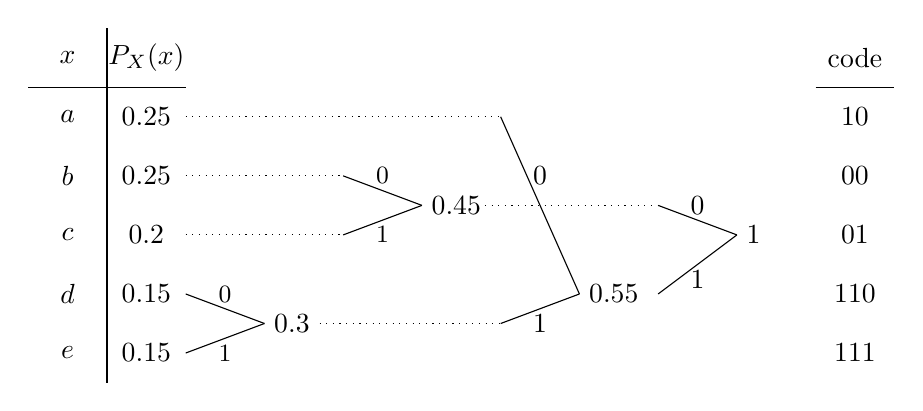
\begin{tikzpicture}
\pgfmathsetmacro{\dist}{0.75}
\node at (0,5*\dist) {$x$};
\node at (0,4*\dist) {$a$};
\node at (0,3*\dist) {$b$};
\node at (0,2*\dist) {$c$};
\node at (0,1*\dist) {$d$};
\node at (0,0*\dist) {$e$};
\draw (-0.5,4.5*\dist) -- (1.5,4.5*\dist);
\draw (0.5,-0.5*\dist) -- (0.5,5.5*\dist);
\node at (1,5*\dist) {$P_X(x)$};
\node at (1,4*\dist) {$0.25$};
\node at (1,3*\dist) {$0.25$};
\node at (1,2*\dist) {$0.2$};
\node at (1,1*\dist) {$0.15$};
\node at (1,0*\dist) {$0.15$};

%STEP 1
\node at (2,0*\dist) {\small $1$};
\node at (2,1*\dist) {\small $0$};
\draw (1.5,0*\dist) -- (2.5,0.5*\dist);
\draw (1.5,1*\dist) -- (2.5,0.5*\dist);
\node[anchor=west] at (2.5,0.5*\dist) {$0.3$};
%\node[anchor=west] at (2.5,2*\dist) {$0.2$};
%\node[anchor=west] at (2.5,3*\dist) {$0.25$};
%\node[anchor=west] at (2.5,4*\dist) {$0.25$};

%STEP 2
\node at (4,2*\dist) {\small $1$};
\node at (4,3*\dist) {\small $0$};
\draw[dotted] (1.5,2*\dist) -- (3.5,2*\dist);
\draw[dotted] (1.5,3*\dist) -- (3.5,3*\dist);
\draw (3.5,2*\dist) -- (4.5,2.5*\dist);
\draw (3.5,3*\dist) -- (4.5,2.5*\dist);
\node[anchor=west] at (4.5,2.5*\dist) {$0.45$};
%\node[anchor=west] at (4.5,0.5*\dist) {$0.3$};
%\node[anchor=west] at (4.5,4*\dist) {$0.25$};

%STEP 3
\node at (6,0.5*\dist) {$1$};
\node at (6,3*\dist) {$0$};
\draw[dotted] (3.2,0.5*\dist) -- (5.5,0.5*\dist);
\draw[dotted] (1.5,4*\dist) -- (5.5,4*\dist);
\draw (5.5,0.5*\dist) -- (6.5,1*\dist);
\draw (5.5,4*\dist) -- (6.5,1*\dist);
%\node[anchor=west] at (6.5,2.5*\dist) {$0.45$};
\node[anchor=west] at (6.5,1*\dist) {$0.55$};

%STEP 4
\node at (8,1.25*\dist) {$1$};
\node at (8,2.5*\dist) {$0$};
\draw[dotted] (5.3,2.5*\dist) -- (7.5,2.5*\dist);
\draw (7.5,2.5*\dist) -- (8.5,2*\dist);
\draw (7.5,1*\dist) -- (8.5,2*\dist);
\node[anchor=west] at (8.5,2*\dist) {$1$};

%RESULT
\node at (10,5*\dist) {code};
\draw (9.5,4.5*\dist) -- (10.5,4.5*\dist);
\node at (10,4*\dist) {$10$};
\node at (10,3*\dist) {$00$};
\node at (10,2*\dist) {$01$};
\node at (10,1*\dist) {$110$};
\node at (10,0*\dist) {$111$};
\end{tikzpicture}
\end{center}
We build up the tree from left to right, pairing the symbols (or groups of symbols) with smallest (combined) probabilities at every step. The codeword for every symbol is then determined by following the branches of the tree \emph{from right to left} until the symbol is reached. Note that this way, the symbols with the smallest probabilities get assigned the longest codewords (paths).

The average codeword length for this code is
\begin{align}
0.25 \cdot 2 + 0.25 \cdot 2 + 0.2 \cdot 2 + 0.15 \cdot 3 + 0.15 \cdot 3 = 2.3. 
\end{align}
Compare this to $H(X) \approx 2.285$. The average codeword length lies between $H(X)$ and $H(X) + 1$.
\end{example}

The above was an example of how to construct \emph{binary} Huffman codes. We can also generate Huffman codes for larger alphabets, resulting in ternary, quaternary, or, more generally, \term{$d$-ary Huffman codes}.

\begin{example}[Ternary Huffman code]\label{example:ter-huffman}
We build a Huffman code with the alphabet $\set{0,1,2}$ for the same distribution as in Example~\ref{example:bin-huffman}.
\begin{center}
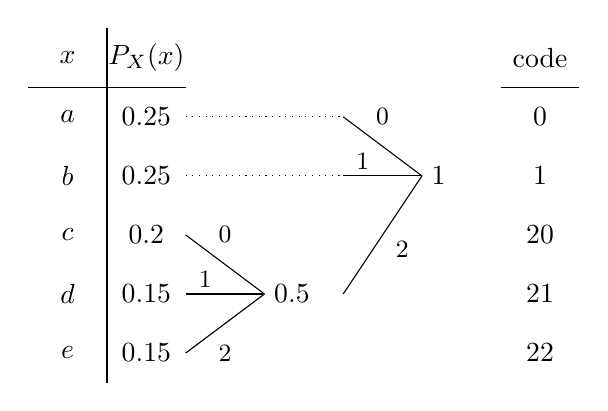
\begin{tikzpicture}
\pgfmathsetmacro{\dist}{0.75}
\node at (0,5*\dist) {$x$};
\node at (0,4*\dist) {$a$};
\node at (0,3*\dist) {$b$};
\node at (0,2*\dist) {$c$};
\node at (0,1*\dist) {$d$};
\node at (0,0*\dist) {$e$};
\draw (-0.5,4.5*\dist) -- (1.5,4.5*\dist);
\draw (0.5,-0.5*\dist) -- (0.5,5.5*\dist);
\node at (1,5*\dist) {$P_X(x)$};
\node at (1,4*\dist) {$0.25$};
\node at (1,3*\dist) {$0.25$};
\node at (1,2*\dist) {$0.2$};
\node at (1,1*\dist) {$0.15$};
\node at (1,0*\dist) {$0.15$};

%STEP 1
\node at (2,0*\dist) {\small $2$};
\node at (1.75,1.25*\dist) {\small $1$};
\node at (2,2*\dist) {\small $0$};
\draw (1.5,0*\dist) -- (2.5,1*\dist);
\draw (1.5,1*\dist) -- (2.5,1*\dist);
\draw (1.5,2*\dist) -- (2.5,1*\dist);
\node[anchor=west] at (2.5,1*\dist) {$0.5$};

%STEP 2
\node at (4.25,1.75*\dist) {\small $2$};
\node at (3.75,3.25*\dist) {\small $1$};
\node at (4,4*\dist) {\small $0$};
\draw (3.5,1*\dist) -- (4.5,3*\dist);
\draw (3.5,3*\dist) -- (4.5,3*\dist);
\draw (3.5,4*\dist) -- (4.5,3*\dist);
\draw[dotted] (1.5,3*\dist) -- (3.5,3*\dist);
\draw[dotted] (1.5,4*\dist) -- (3.5,4*\dist);
\node[anchor=west] at (4.5,3*\dist) {$1$};

%RESULT
\node at (6,5*\dist) {code};
\draw (5.5,4.5*\dist) -- (6.5,4.5*\dist);
\node at (6,4*\dist) {$0$};
\node at (6,3*\dist) {$1$};
\node at (6,2*\dist) {$20$};
\node at (6,1*\dist) {$21$};
\node at (6,0*\dist) {$22$};
\end{tikzpicture}
\end{center}
\end{example}

\begin{exercise}\label{exercise:ter-huffman}
Use the above procedure to construct a ternary code for the source $X$ with $\mathcal{X} = \set{a,b,c,d,e,f}$ and $P_X(a) = P_X(b) = 0.25$, $P_X(c) = 0.2$, $P_X(d) = P_X(e) = P_X(f) = 0.1$. Can you find another code with a smaller average codeword length?
\end{exercise}
We have to be careful, because with an alphabet size of greater than 2, the above procedure does not always give an optimal code! In fact, a $d$-ary code is only optimal if $|\mathcal{X}|$ is of the form $k(d-1)+1$ for some $k \in \mathbb{N}$. This ensures that at every step, we can combine exactly $d$ symbols to use the alphabet at full capacity. The ternary code in Example~\ref{example:ter-huffman} is optimal because $|\mathcal{X}| = 5 = 2(3-1) + 1$, but the code you constructed in Exercise~\ref{exercise:ter-huffman} is not. To remedy this, one can add one or more `dummy' symbols to the source (each with probability zero) until an appropriate size of $\mathcal{X}$ is reached. The codewords for those dummy symbols are discarded at the end.

We now show that Huffman codes indeed produce an optimal code length.

\begin{theorem}[Optimality of Huffman codes]
Let $X$ be a source, and let $C^*$ be the associated Huffman code. For any other uniquely decodable code $C'$ with the same alphabet,
\[
\len_{C^*}(X) \leq \len_{C'}(X).
\]
\end{theorem}
\begin{proof}[Proof (sketch)]
We sketch the proof for binary codes. The proof idea extends to any alphabet size.

Let $a,b \in \mathcal{X}$ be the two symbols with lowest probability, and $P_X(a) \leq P_X(b)$. Suppose, for some prefix-free code $C'$, that $\len_a < \len_b$. We can be in one of two cases:
\begin{enumerate}
\item $\len_b$ is not the maximal codeword length. In other words, some $c$ exists with $P_X(c) \geq P_X(a)$ and $\len_c > \len_a$.
\item $\len_b$ is the maximal codeword length. Then there exists a `sibling' $c$ in the code tree such that $\len_c = \len_b$ (if not, we can remove the last bits of the code for $b$ by prefix-freeness). For this $c$, $P_X(c) \geq P_X(a)$ and $\len_c > \len_a$.
\end{enumerate}
In both cases, we can swap the codewords for $a$ and $c$, achieving a code that is at least as efficient as $C'$. Therefore, we may assume that for all source symbols $x_i, x_j \in \mathcal{X}$ with $P_X(x_i) \leq P_X(x_j)$, $\len_{x_i} \geq \len_{x_j}$.

Using this assumption, we can transform any code $C'$ into a Huffman code using induction on the size of the source. The full proof can be found in \CT{} (Theorem 5.8.1).
\end{proof}

\begin{example}[20 questions]
In the game of `20 questions' (20Q), the goal is to identify an object from a set of objects using (at most) 20 yes/no questions. Assume we know the probability distribution $P_X$ over all possible objects. We can view the sequence of questions as the `code' for an object \yfke{Your blackboard photo says it's the sequence of questions, but I don't understand: it's still a binary tree right? So the code seems to be the sequence of answers (yes/no).}: the number of questions asked is the length of the codeword. By Shannon's source coding theorem,
\[
H(X) \leq \mbox{expected number of questions} \leq H(X) + 1,
\]
and the Huffman code procedure can be used to determine the optimal sequence of questions.
\end{example}
As we have seen, the average codeword length of Huffman codes is theoretically optimal. However, Huffman codes (and symbol codes in general) still have a number of disadvantages:
\begin{itemize}
\item When compressing, for example, an English text symbol-by-symbol, the probability distribution for each position may depend on the string of text that precedes it: for example, the letter \texttt{n} is a lot more likely than the letter \texttt{a} if it comes after the string \texttt{informatio}. Given this change of distribution, the Huffman code may not produce the shortest possible code. This can be resolved by recomputing the Huffman code after every symbol, but this results in a lot of overhead.
\item The average codeword length is upper bounded by $H(X) + 1$. This is fine when $H(X)$ is very large, but can be a significant overhead when $H(X)$ is small.
\end{itemize}

\section{Arithmetic codes}
In this section, we study a different kind of code that can handle context-dependent distributions, unlike the Huffman code.

\begin{definition}[Standard binary representation]
The standard binary representation of a real number $r \in [0,1)$ is a (possibly infinite) string of bits $c_1c_2\cdots$ such that
\[
r = \sum_i c_i \cdot 2^{-i},
\]
where by convention, 0 is represented by the string 0.
\end{definition}
For example, $\frac{1}{2}$ is represented by $1$, $\frac{1}{4}$ by $01$, $\frac{11}{32}$ by $01011$ (note also that $01011$ represents the natural number 11), and $\frac{1}{3}$ by $010101\cdots$. Not all reals in $[0,1)$ have a finite representation, but any interval $[a,b)$ with $0 \leq a < b \leq 1$ contains at least one number with a finite binary representation.

\begin{definition}[Arithmetic code]\label{def:arithmetic}
Given a source $P_X$ with $\mathcal{X} = \{x_1, .., x_m\}$, construct the arithmetic code as follows. Divide the interval $[0,1)$ into disjoint subintervals $I_{x_j} = [a_j, b_j)$ (for $1 \leq j \leq m$) such that $b_j - a_j = P_X(x_j)$, and $a_j = b_{j-1}$ (and $a_1 = 0, b_m = 1$).

The encoding $AC(x_j)$ of the element $x_j$ is the (shortest possible) standard binary representation of some number in $I_{x_j}$. 
\end{definition}

\begin{example}\label{example:arithmetic}
Let $X$ be a random variable with $\mathcal{X} = \set{1,2,3}$ and $P_X(1) = \frac{1}{2}$, $P_X(2) = P_X(3) = \frac{1}{4}$. The arithmetic code is constructed by first determining the intervals:
\begin{center}
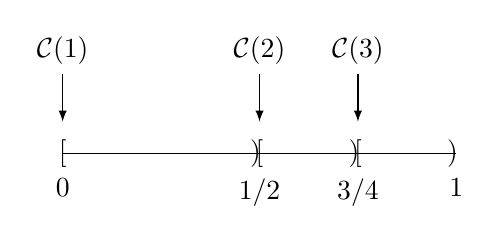
\begin{tikzpicture}
\draw (0,0) -- (5,0);
\draw node at (0,0) {$[$};
\draw node at (2.5,0) {$[$};
\draw node at (3.75,0) {$[$};
\draw node at (2.45,0) {$)$};
\draw node at (3.7,0) {$)$};
\draw node at (4.95,0) {$)$};
\draw[anchor=north] node at (0,-0.2) {$0$};
\draw[anchor=north] node at (2.5,-0.2) {$1/2$};
\draw[anchor=north] node at (3.75,-0.2) {$3/4$};
\draw[anchor=north] node at (5,-0.2) {$1$};
%
\draw[-latex] (0,1) -- (0,0.4);
\draw[-latex] (2.5,1) -- (2.5,0.4);
\draw[-latex] (3.75,1) -- (3.75,0.4);
\draw[anchor=south] node at (0,1) {$\mathcal{C}(1)$};
\draw[anchor=south] node at (2.5,1) {$\mathcal{C}(2)$};
\draw[anchor=south] node at (3.75,1) {$\mathcal{C}(3)$};
\end{tikzpicture}
\end{center}
This image results in the arithmetic code $\mathcal{C}$ with $\mathcal{C}(1) = 0$ (the representation of 0), $\mathcal{C}(2) = 1$ (the representation of $\frac{1}{2}$), $\mathcal{C}(2) = 11$ (the representation of $\frac{3}{4}$).

For $X$, the codewords happen to fall exactly \emph{on} the boundaries of the intervals. This is not always the case, however. The same code would have resulted from this procedure if we started with the random variable $Y$ with $\mathcal{Y} = \set{1,2,3}$ and $P_Y(1) = P_Y(2) = 0.3$ and $P_Y(3) = 0.4$:

\begin{center}
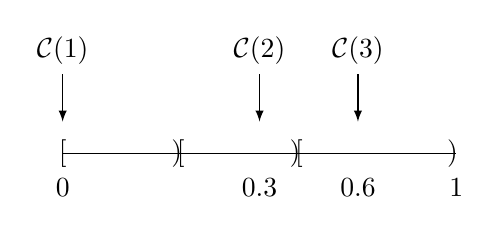
\begin{tikzpicture}
\draw (0,0) -- (5,0);
\draw node at (0,0) {$[$};
\draw node at (1.5,0) {$[$};
\draw node at (3,0) {$[$};
\draw node at (1.45,0) {$)$};
\draw node at (2.95,0) {$)$};
\draw node at (4.95,0) {$)$};
\draw[anchor=north] node at (0,-0.2) {$0$};
\draw[anchor=north] node at (2.5,-0.2) {$0.3$};
\draw[anchor=north] node at (3.75,-0.2) {$0.6$};
\draw[anchor=north] node at (5,-0.2) {$1$};
%
\draw[-latex] (0,1) -- (0,0.4);
\draw[-latex] (2.5,1) -- (2.5,0.4);
\draw[-latex] (3.75,1) -- (3.75,0.4);
\draw[anchor=south] node at (0,1) {$\mathcal{C}(1)$};
\draw[anchor=south] node at (2.5,1) {$\mathcal{C}(2)$};
\draw[anchor=south] node at (3.75,1) {$\mathcal{C}(3)$};
\end{tikzpicture}
\end{center}

\end{example}


\begin{proposition}\label{prop:arithmetic-length}
For any $X$, the arithmetic code has average length $\len_{AC}(X) \leq H(X) + 1$.
\end{proposition}
\begin{proof}
Let $x \in \mathcal{X}$, and define $\len_x := \lceil \log (1/P_X(x))\rceil$. Then
\begin{align}
2^{-\len} = 2^{-\lceil \log (1/P_X(x))\rceil} \leq 2^{-\log (1/P_X(x))} = 2^{\log P_X(x)} = P_X(x).
\end{align}
Therefore, since the size of the interval $I_x$ is $P_X(x)$, there must be some $0 \leq s < 2^\len$ such that $\frac{s}{2^{-\len}}$ lies within $I_x$. This number has binary representation of length $\len \leq -\log P_X(x) + 1$. Thus,
\begin{align}
\len_AC(X) = \mathbb{E}[\len(AC(X))] = \sum_x P_X(x) \len(AC(x)) \leq \sum_x P_X(x) (-\log P_X(x) + 1) = H(X) + 1.
\end{align}
\end{proof}

As we can see from Example~\ref{example:arithmetic}, this construction for arithmetic codes do not necessarily result in a prefix-free code. However, at the expense of one extra bit of code (on average), the construction can be adapted into a prefix-free code. One example of this is the \term{Shannon-Fano-Elias code} (see \CT, Section 5.9), which provides a more sophisticated way of selecting a number within each interval than simply selecting the number with the shortest binary representation. This alternative selection procedure ensures prefix-freeness. Another option is to select \emph{binary intervals} within each interval:

\begin{definition}[Binary interval]
A binary interval is an interval of the form
\[
\left[\frac{s}{2^{\len}}, \frac{s+1}{2^{\len}}\right)
\]
with $s, \len \in \mathbb{N}$ and $0 \leq s < 2^{\len}$. The \term{name} of the interval is the binary representation of $s$ (as a natural number) padded with zeroes on the left to reach length $\len$.
\end{definition}

\begin{definition}[Arithmetic code (prefix-free version)]
The prefix-free arithmetic code is identical to Definition~\ref{def:arithmetic}, except that the encoding $AC^{pf}(x_j)$ of the element $x_j$ is now the name of the largest binary interval that fits entirely in $I_{x_j}$.
\end{definition}
Similarly to Proposition~\ref{prop:arithmetic-length}, it can be shown that for any source  $X$, $\len_{AC^{pf}}(X) \leq H(X) + 2$. Note that we get prefix-freeness only at the expense of an extra bit on average.

\begin{example}
Let $Y$ be the random variable as in Example~\ref{example:arithmetic}, that is, $P_Y(1) = P_Y(2) = 0.3$ and $P_Y(3) = 0.4$. The prefix-free code for $Y$ is constructed as follows:

\begin{center}
\begin{tikzpicture}
\filldraw[draw=none,fill=ocre,opacity=0.5] (0,-0.25) rectangle (1.25,0.25);
\filldraw[draw=none,fill=ocre,opacity=0.5] (1.875,-0.25) rectangle (2.5,0.25);
\filldraw[draw=none,fill=ocre,opacity=0.5] (3.75,-0.25) rectangle (5,0.25);
%
\draw (0,0) -- (5,0);
\draw node at (0,0) {$[$};
\draw node at (1.5,0) {$[$};
\draw node at (3,0) {$[$};
\draw node at (1.45,0) {$)$};
\draw node at (2.95,0) {$)$};
\draw node at (4.95,0) {$)$};
\draw[anchor=north] node at (0,-0.2) {$0$};
\draw[anchor=north] node at (2.5,-0.2) {$0.3$};
\draw[anchor=north] node at (3.75,-0.2) {$0.6$};
\draw[anchor=north] node at (5,-0.2) {$1$};
%
\draw[dotted] (0,0) -- (0,0.5);
\draw[dotted] (1.25,0) -- (1.25,0.5);
\draw[dotted] (1.875,0) -- (1.875,0.5);
\draw[dotted] (2.5,0) -- (2.5,0.5);
\draw[dotted] (3.75,0) -- (3.75,0.5);
\draw[dotted] (5,0) -- (5,0.5);
\draw[anchor=south] node at (0,0.5)     {$\frac{0}{4}$};
\draw[anchor=south] node at (1.25,0.5)  {$\frac{1}{4}$};
\draw[anchor=south] node at (1.875,0.5) {$\frac{3}{8}$};
\draw[anchor=south] node at (2.5,0.5)   {$\frac{4}{8}$};
\draw[anchor=south] node at (3.75,0.5)  {$\frac{3}{4}$};
\draw[anchor=south] node at (5,0.5)     {$\frac{4}{4}$};
\end{tikzpicture}
\end{center}
This results in the codewords $\mathcal{C}(1) = 00$, $\mathcal{C}(2) = 011$, and $\mathcal{C}(3) = 11$.
\end{example}
The arithmetic code is slightly less efficient than the Huffman code in terms of average codeword length. A big advantage is the way it is able to adapt to changing distributions, such as when we are encoding a stream of English text. Suppose we are given the (not necessarily i.i.d.) random variables $X_1, X_2, ..., X_n$, and we want to encode the source $X_1X_2 \cdots X_n$. We start by dividing the interval $[0,1)$ into subintervals according to $P_{X_1}$. If, for example, the event $X_1 = b$ happens, we zoom into the interval corresponding to $b$, and subdivide \emph{that} interval according to $P_{X_2|X_1}$, so that the sizes of these intervals add up to $P_{X_1}(b)$. This principle is used in the keyboard alternative \href{http://wol.ra.phy.cam.ac.uk/djw30/dasher/}{Dasher}.

\section{Asymptotic Equipartition Property (AEP)}
\newcommand{\convto}{\xrightarrow{n \to \infty}}
\newcommand{\convtoP}{\xrightarrow{p}}
\newcommand{\convtoMS}{\xrightarrow{m.s.}}
\newcommand{\convtoAS}{\xrightarrow{a.s.}}
\newcommand{\typset}{A_{\epsilon}^{(n)}}
\newcommand{\typsetp}{A_{\epsilon'}^{(n)}}
\newcommand{\typsetb}{B_{\delta}^{(n)}}


In this section, we consider the possibility of encoding blocks of symbols, rather than just one symbol at at time. We restrict our attention to sources that are \emph{real} random variables. The following definition of converging random variables may remind you of a converging sequence of numbers. Recall that a sequence $x_1, x_2, x_3, ...$ of numbers converges to $x$ if $\forall\epsilon > 0 \ \exists n_0 \ \forall (n \geq n_0) : |x_n - x| < \epsilon$. We denote this by writing $x_n \convto x$.
\begin{definition}[Converging random variables]
A sequence $X_1, X_2, X_3, ...$ of real random variables converges to a random variable $X$, if it satisfies one of the following definitions:
\begin{tabular}{l l l}
\term{in probability} & (notation $X_n \convtoP X$)  & if $\forall \epsilon > 0$, $P[|X_n - X| > \epsilon] \convto 0$\\
\term{in mean square} & (notation $X_n \convtoMS X$) & if $\mathbb{E}[(X_n - X)^2] \convto 0$\\
\term{almost surely}  & (notation $X_n \convtoAS X$) & if $P[\lim_{n \to \infty} X_n = X|] = 1$ 
\end{tabular}
\\where the definition of $X_n \convtoAS X$ can be interpreted as $P[\set{\omega \in \Omega \mid X_n(\omega) \convto X(\omega)}] = 1$.
\end{definition}

\yfke{maybe add example here?}


In general, the following implications hold (although their converses do not):
\begin{align}
X_n \convtoMS X \ \ \ &\Rightarrow\ \ \  X_n \convtoP X\\
X_n \convtoAS X \ \ \ &\Rightarrow\ \ \  X_n \convtoP X
\end{align}
The following well-known law states that if we sample several times from the same distribution, the average converges (in probability) to the expected value of the distribution.
\begin{theorem}[Weak Law of Large Numbers]
Let $X_1, X_2, ...$ be real i.i.d. random variables with mean $\mu = \mathbb{E}[X_i]$ and variance $\sigma^2 = \mathbb{E}[(X_i - \mu)^2] < \infty$. Define the random variables
\[
S_n := \frac{1}{n} \sum_{i=1}^n X_i.
\]
Then $S_n \convtoP \mu$.
\end{theorem}
This important law has an entropy variant, which follows almost directly:
\begin{theorem}[Asymptotic Equipartition Property (AEP)]
Let $X_1, X_2, X_3, ...$ be real i.i.d. random variables with distribution $P_X$. Then
\[
-\frac{1}{n} \log P_{X_1 \cdots X_n}(X_1, ..., X_n) \convtoP H(X).
\]
(Note that $P_{X_1 \cdots X_n}(X_1, ..., X_n)$ is itself a random variable, and $H(X)$ can be regarded as a constant random variable.)
\end{theorem}
\begin{proof}
Since the variables $X_i$ are independent, so are the random variables $\log P_X(X_i)$. Then
\begin{align}
-\frac{1}{n} \log P_{X_1\cdots X_n}(X_1, ..., X_n) &= -\frac{1}{n} \sum_{i=1}^n \log P_X(x_i)\nonumber\\
&\convtoP - \mathbb{E}[\log P_X(X_i)] = H(X)
\end{align}
by the weak law of large numbers.
\end{proof}

%\begin{example}[Biased coin flip]
%Consider flipping a biased coin, with probability of 1 (heads) being $p_1 = 0.1$ and probability of 0 (tails) being $p_0 = 0.9$. (This is an example of a \term{Bernoulli distribution} with success probability $p_1$ and failure probability $p_0 = 1 - p_1$.) We can compute that $H(X) = h(0.1) \approx 0.469$.
%
%Clearly, for every $n$, $P_{X_1 \cdots X_n}(x_1\cdots x_n) = p_0^{n-r(x)}p_1^{r(x)}$, where $r(x)$ is the number of ones in the string $x = x_1\cdots x_n$. In particular, this gives us the \term{binomial distribution} by considering the random variable $R = r(X_1, ..., X_n)$, since $P(r) = \binom{n}{r} p_0^{n-r} p_1^r$.
%\end{example}

\begin{definition}[Typical set]
A typical set $\typset$ with respect to $P_X$ is the set of strings $(x_1, ..., x_n) \in {\cal X}^n$ such that
\[
2^{-n (H(X) + \epsilon)} \leq P_{X^n}(x_1, ..., x_n) \leq 2^{-n(H(X) - \epsilon)}.
\]
\end{definition}
The typical set is relatively small, but contains almost all of the probability mass. We start by establishing some general properties of typical sets.

\begin{proposition}\label{prop:typset-properties}
A typical set $\typset$ satisfies the following:
\begin{enumerate}
\item For all $(x_1, ..., x_n) \in \typset$, \[H(X) - \epsilon \leq - \frac{1}{n} \log P_{X^n}(x_1, ..., x_n) \leq H(X) + \epsilon.\]
\item $P[\typset] > 1 - \epsilon$ (for large enough $n$).
\item $|\typset| \leq 2^{n(H(X) + \epsilon)}$
\item $|\typset| \geq (1-\epsilon) 2^{n(H(X) - \epsilon)}$ (for large enough $n$).
\end{enumerate}
\end{proposition}
\begin{proof}\ 
\begin{enumerate}
\item This is immediate from the definition (take the logarithm and divide by $-n$).
\item This follows from the Asymptotic Equipartition Property: for all $\epsilon > 0$, $P[|-\frac{1}{n} \log P_{X^n}(X_1, ..., X_n) - H(X)| > \epsilon] \convto 0$, that is,
\begin{align}\forall (\epsilon > 0) \ \forall (\delta > 0) \ \exists n_0 \ \forall (n \geq n_0) \ P[|-\frac{1}{n} \log P_{X^n}(X_1, ..., X_n) - H(X)| \leq \epsilon] > 1 - \delta.
\end{align}
By choosing $\delta := \epsilon$, the result follows from the first property.
\item First, observe that
\begin{align}
1 = \sum_{\vec{x} \in \mathcal{X}^n} P_{X^n}(\vec{x}) \geq \sum_{\vec{x} \in \typset} P_{X^n}(\vec{x}) \geq |\typset| \cdot 2^{-n(H(X) + \epsilon},
\end{align}
where the last inequality follows by property 1. The result now follows by multiplying both sides of the equation by $2^{n(H(X) + \epsilon)}$.
\item By property 2, we can choose an $n$ large enough so that
\begin{align}
1 - \epsilon < P[\typset] = \sum_{\vec{x} \in \typset} P_{X^n}(\vec{x}) \leq |\typset| \cdot 2^{-n(H(X)-\epsilon)},
\end{align}
where again, the last inequality follows by property 1.
\end{enumerate}
\end{proof}


Typical sets and their properties allow us to code a source $X$, $n$ symbols at a time, in either a lossy or a lossless way. For a lossy code, simply assign binary labels of length (at most) $\lceil n (H(X) + \epsilon)\rceil$ to the elements of $\typset$, and assign some constant (dummy) codeword to all elements outside of the set. Decoding this dummy codeword will result in an error (data loss), but this error occurs with probability at most $\epsilon$.

The above scheme can be extended to a lossless version by assigning longer labels to the elements outside of $\typset$, for example binary labels of length $\lceil \log |\mathcal{X}|^n\rceil = \lceil n \log |\mathcal{X}|\rceil$. An extra `flag' bit is needed to indicate whether the element is inside or outside the typical set. For large enough $n$, this code is quite efficient:
\begin{theorem}
Let $X_1, ..., X_n$ be i.i.d. real random variables with respect to the set $\mathcal{X}$, and distributed according to $P_X$. Let $\epsilon > 0$. Then there exists a lossless code $\mathcal{X}^n \to \{0,1\}^*$ such that, for sufficiently large $n$, $\mathbb{E}[\frac{1}{n} \len(X^n)] \leq H(X) + \epsilon$.
\end{theorem}
\begin{proof}
Consider the code described above: the code consist of a flag bit (indicating whether or not the element is inside the typical set), followed by either a short label (for elements in the typical set) or a longer one (for elements outside of it).

Let $\epsilon' > 0$ (we will specify the value of $\epsilon'$ later). Let $n$ be large enough such that $P[\typsetp] > 1 - \epsilon'$ (see Proposition~\ref{prop:typset-properties}). Then
\begin{align}
\mathbb{E}[\len(X^n)] &= \sum_{\vec{x} \in \mathcal{X}^n} P_{X^n}(\vec{x}) \len(\vec{x})\nonumber\\
&= \sum_{\vec{x} \in \typsetp} P_{X^n}(\vec{x}) \len(\vec{x}) + \sum_{\vec{x} \not\in \typsetp} P_{X^n}(\vec{x}) \len(\vec{x})\nonumber\\
&\leq P[\typsetp] \cdot (\lceil n (H(X) + \epsilon') \rceil + 1) + P[\overline{\typsetp}] \cdot (\lceil n \log |\mathcal{X}| \rceil + 1)\nonumber\\
&\leq P[\typsetp] \cdot (n (H(X) + \epsilon') + 2) + P[\overline{\typsetp}] \cdot (n \log |\mathcal{X}| + 2)\nonumber\\
&\leq n ( H(X) + \epsilon') + \epsilon' \cdot n \log |\mathcal{X}| + 2\nonumber\\
&= n(H(X) + \epsilon'),
\end{align}
where $\epsilon = \epsilon' + \epsilon' \log |\mathcal{X}| + \frac{2}{n}$ (note that $\epsilon$ can be made arbitrarily small by choosing $\epsilon'$ and $n$ wisely). The +1 in the first inequality is a consequence of the `flag' bit.
\end{proof}
For large enough blocks of symbols, typical sets thus allow the construction of an efficient code without the 1 bit of overhead that symbol codes may necessarily have. However, this efficiency is only guaranteed for `sufficiently large $n$', a rather theoretical condition that may not be achievable in practice.

We conclude this chapter by showing that the typical set is in a sense `optimal', i.e. that picking a smaller set instead of the typical set does not allow for much shorter codewords on average in a lossy setting, not even if we allow rather large error probabilities by allowing about half of the elements to lie outside of the typical set.

Let us use the notation $\typsetb$ to denote the smallest subset of $\mathcal{X}^n$ such that $P[\typsetb] > 1 - \delta$ (for some parameter $\delta > 0$). $\typsetb$ can be explicitly constructed by, for example, ordering $\mathcal{X}^n$ in order of decreasing probability, and adding elements to $\typsetb$ until the probability threshold of $1 - \delta$ is reached. The following theorem states that even for large values of $\delta$, we still need almost $n H(X)$ bits to denote an element from $\typsetb$.

\begin{theorem}
Let $X_1, ..., X_n$ be i.i.d. random variables distributed according to $P_X$. For any $\delta < \frac{1}{2}$, and any $\delta' > 0$, if $P[\typsetb] > 1 - \delta$, then
\[
\frac{1}{n} \log |\typsetb| > H(X) - \delta',
\]
for sufficiently large $n$.
\end{theorem}
\begin{proof}
Let $\delta,\epsilon < \frac{1}{2}$, and consider some $\typsetb$ such that $P[\typsetb] > 1 - \delta$. We know that by Proposition~\ref{prop:typset-properties}, $P[\typset] > 1 - \epsilon$, for large enough $n$. Thus, by the union bound,
\begin{align}
1 - \epsilon - \delta &< 1 - P[\overline{\typset}] - P[\overline{\typsetb}]\
&\leq P[\typset \cap \typsetb]\nonumber\\
&= \sum_{\vec{x} \in \typset \cap \typsetb} P_{X^n}(\vec{x})\nonumber\\
&\leq \sum{\vec{x} \in \typset \cap typsetb} 2^{-n(H(X) - \epsilon}\nonumber\\
&= |\typset \cap \typsetb| \cdot 2^{-n}(H(X) - \epsilon)\nonumber\\
&\leq |\typsetb| \cdot 2^{-n}(H(X) - \epsilon).
\end{align}
Rearranging this expression and taking the logarithm, we get
\begin{align}
H(X) - \epsilon + \frac{1}{n} \log (1 - \epsilon - \delta) < \frac{1}{n} \log |\typsetb|.
\end{align}
If we now set $\delta' := \epsilon - \frac{1}{n} \log (1 - \epsilon - \delta)$, then
\begin{align}
H(X) - \delta' < \frac{1}{n} \log |\typsetb|,
\end{align}
as desired.
\yfke{I'm not sure what happens to $\delta'$ here: the proof should work for any $\delta' > 0$, aren't we restricting the freedom here? Or can we always find an epsilon to accommodate for the values of $\delta$ and $\delta'$ that are given?}
\end{proof}
